% \iffalse
\let\negmedspace\undefined
\let\negthickspace\undefined
\documentclass[journal,12pt,twocolumn]{IEEEtran}
\usepackage{cite}
\usepackage{amsmath,amssymb,amsfonts,amsthm}
\usepackage{algorithmic}
\usepackage{graphicx}
\usepackage{textcomp}
\usepackage{xcolor}
\usepackage{txfonts}
\usepackage{listings}
\usepackage{enumitem}
\usepackage{mathtools}
\usepackage{gensymb}
\usepackage{comment}
\usepackage{tikz}
\usepackage[breaklinks=true,hidelinks]{hyperref}
\usepackage{tkz-euclide} 
\usepackage{listings}
\usepackage{gvv}
\def\inputGnumericTable{}
\usepackage[latin1]{inputenc}                              
\usepackage{color} 
\usepackage{array}                                            
\usepackage{longtable}                                       
\usepackage{calc}                                             
\usepackage{multirow}                                         
\usepackage{hhline}                                           
\usepackage{ifthen}                                           
\usepackage{lscape}

\newtheorem{theorem}{Theorem}[section]
\newtheorem{problem}{Problem}
\newtheorem{proposition}{Proposition}[section]
\newtheorem{lemma}{Lemma}[section]
\newtheorem{corollary}[theorem]{Corollary}
\newtheorem{example}{Example}[section]
\newtheorem{definition}[problem]{Definition}
\newcommand{\BEQA}{\begin{eqnarray}}
\newcommand{\EEQA}{\end{eqnarray}}
\newcommand{\define}{\stackrel{\triangle}{=}}
\theoremstyle{remark}
\newtheorem{rem}{Remark}
\begin{document}

\bibliographystyle{IEEEtran}
\vspace{3cm}

\title{DISCRETE 11.9.4 Q-1}
\author{EE23BTECH11207 -KAILASH.C$^{*}$% <-this % stops a space
}
\maketitle
\newpage
\bigskip

\renewcommand{\thefigure}{\theenumi}
\renewcommand{\thetable}{\theenumi}


Find the sum of n terms of the series:
$1\times2+2\times3+3\times4+4\times5+....$\\
\solution
\fi
\begin{table}[h]
\begin{tabular}{|l|l|}
\hline
\textbf{Symbols} & \textbf{Definition}\\ \hline
$x\brak{n}$ & General term \\ \hline
$y\brak{n}$ & Sum of terms till $n_{th}$term \\ \hline
$Y\brak{z}$ & Z-Transformation Of $y\brak{n}$\\ \hline
\end{tabular}
\caption{Parameter Table}
\label{tab:ncert 11.9.4.1}
\end{table}


\begin{align}
 x\brak{n}&=\brak{n+1}\brak{n+2}u\brak{n}\label{eq:11.9.4.1.1}
\end{align}
By Z-transformation property:
\begin{align}
Z\sbrak{nf\brak{n}}=-z\frac{d}{dz}F\brak{z}\label{eq:11.9.4.1.2}
\end{align}
By \eqref{eq:11.9.4.1.2},We have the formulas for:
\begin{align}
nu\brak{n}&\xleftrightarrow[]{Z} \frac{z^{-1}}{\brak{1-z^{-1}}^2}\label{eq:11.9.4.1.3}\\
n^2u\brak{n}&\xleftrightarrow[]{Z}\frac{z^{-1}\brak{z^{-1}+1}}{\brak{1-z^{-1}}^3}\label{eq:11.9.4.1.4}
\end{align}
Using \eqref{eq:11.9.4.1.3},\eqref{eq:11.9.4.1.4} for z-transformation of $x\brak{n}$
\begin{align}
    X\brak{z}&=\frac{z^{-1}\brak{z^{-1}+1}}{\brak{1-z^{-1}}^3}+\frac{3z^{-1}}{\brak{1-z^{-1}}^2}+\frac{2}{1-z^{-1}},\quad\abs{z}>\abs{1}\label{eq:11.9.4.1.5}\\
    Y\brak{z}&=X\brak{z}*U\brak{z}\label{eq:11.9.4.1.6}\\
   &=\brak{\frac{z^{-1}\brak{z^{-1}+1}}{\brak{1-z^{-1}}^3}+\frac{3z^{-1}}{\brak{1-z^{-1}}^2}+\frac{2}{1-z^{-1}}}\frac{1}{1-z^{-1}}\label{eq:11.9.4.1.7}\\
   &=\frac{z^{-1}\brak{z^{-1}+1}}{\brak{1-z^{-1}}^4}+\frac{3z^{-1}}{\brak{1-z^{-1}}^3}+\frac{2}{\brak{1-z^{-1}}^2}\label{eq:11.9.4.1.8}
\end{align}
By using inverse Z transformation,we have:
\begin{align}
    \frac{z^{-1}\brak{z^{-1}+1}}{\brak{1-z^{-1}}^4}&\xleftrightarrow[]{Z^{-1}} \frac{2n^3-3n^2+n}{6}\label{eq:11.9.4.1.9}\\
    \frac{3z^{-1}}{\brak{1-z^{-1}}^3}&\xleftrightarrow[]{Z^{-1}} \frac{3n^2+3n}{2}\label{eq:11.9.4.1.10}\\
    \frac{2}{\brak{1-z^{-1}}^2}&\xleftrightarrow[]{Z^{-1}} n^2+2n+2\label{eq:11.9.4.1.11}
\end{align}
By adding \eqref{eq:11.9.4.1.9},\eqref{eq:11.9.4.1.10} and \eqref{eq:11.9.4.1.11},we get:
\begin{align}
    y\brak{n}&=\frac{2n^3+12n^2+22n+12}{6}\label{eq;11.9.4.1.12}\\
    &=\frac{n^3+6n^2+11n+6}{3}\label{eq:11.9.4.1.13}\\
    &=\frac{\brak{n+1}\brak{n+2}\brak{n+3}}{3}\label{eq:11.9.4.1.14}
\end{align}
\begin{figure}[h]
        \centering
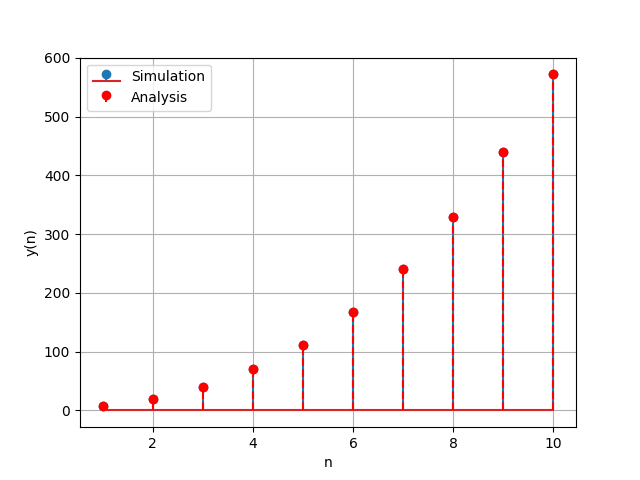
\includegraphics[width=\columnwidth]{Graph.png}
    \caption{Simulation v/s Analysis}
    \label{fig:plot11.9.4.1}
\end{figure}
\end{document}

